
\subsection{Distributed File Sharing}

\subsubsection*{Hash Tree}

The hash tree of a given directory is a tree object that stores information about its structure and contents. This is used to tell users what information they need to download, where it goes and what its contents should be. For every file, the hash tree stores a series of SHA-256 hashes. 

\begin{figure}[ht]
  \centering
  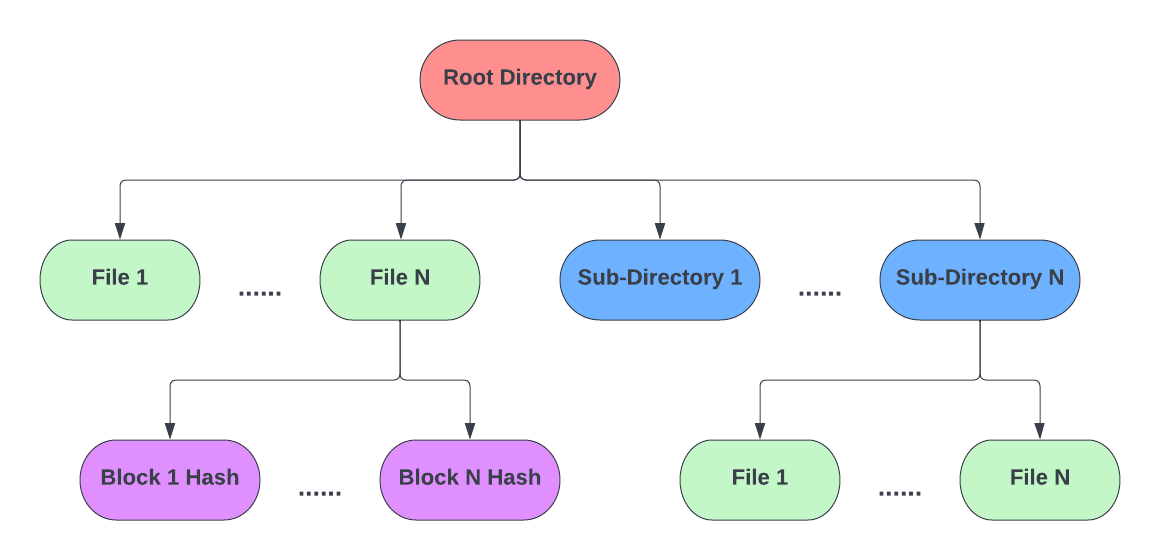
\includegraphics[width=.85\textwidth]{assets/images/diagrams/block-body.png}
  \caption{THe structure of a hash tree}
  \label{fig:hash-storage}
\end{figure}

\subsubsection*{Uploading Content}

For a developer to upload their game (\textbf{F\_M5}) they must provide the required metadata outlined in Section~\ref{subsubsec:eth-data} as well as a hash tree that is generated when they create the game.
\x
A developer is expected to host their hash tree on IPFS indefinitely and seed the game data at least to an initial group of people. 

\subsubsection*{Downloading Content}

\subsubsection*{Updating Content}

\subsubsection*{Downloadable Content}

\subsubsection*{Proving Contribution}